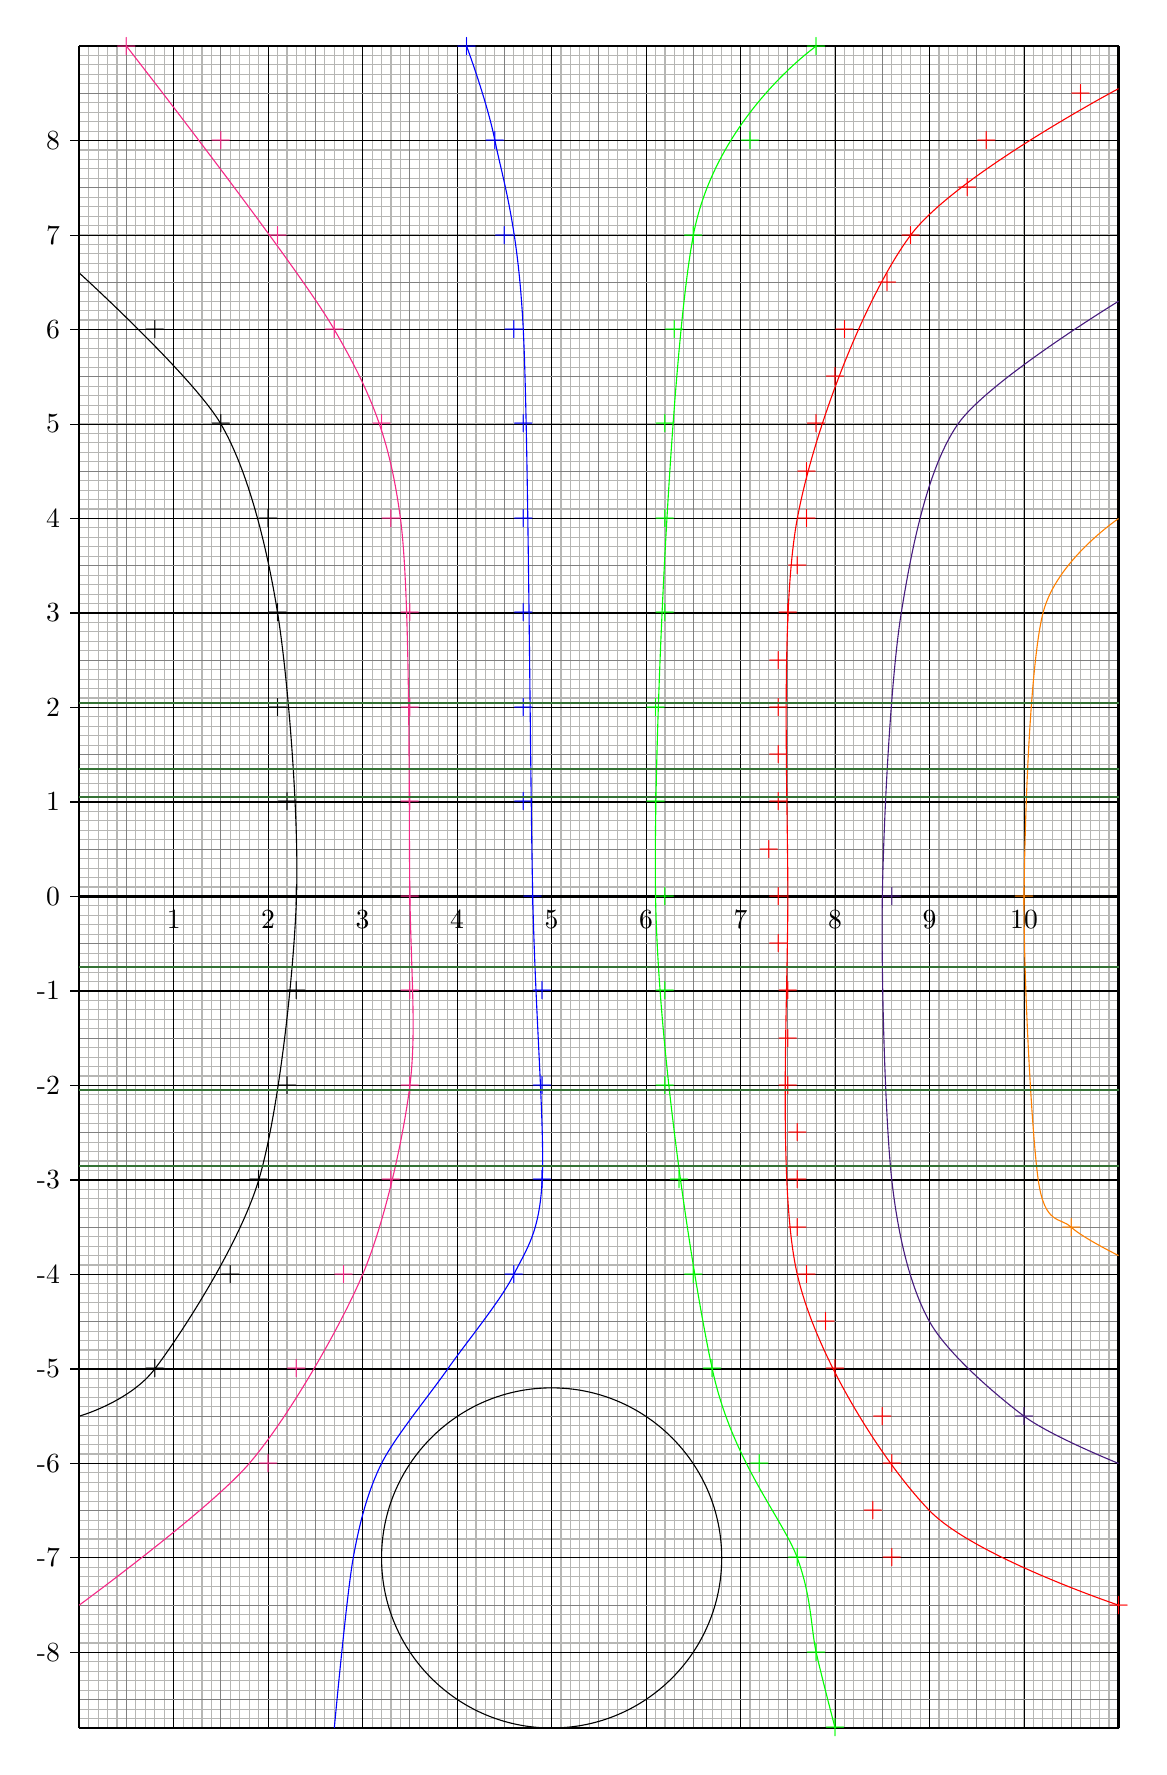
\begin{tikzpicture}[xscale=1.2,yscale=1.2]
		
		\definecolor{cyan}{HTML}{0000FF}
		\definecolor{pink}{HTML}{F52887}
		\definecolor{green}{HTML}{00FF00}
		\definecolor{purple}{HTML}{461B7E}
		\definecolor{taupe}{HTML}{347235}
		\definecolor{grey}{HTML}{B6B6B4}

		
		% Gitter
		\foreach \x in {0.1,0.2,...,11} \draw[- ,grey ,thin] (\x,-8.8) -- (\x,9);
		\foreach \y in {-8.8,-8.7,...,9} \draw[- ,grey ,thin] (0,\y) -- (11,\y);
		\foreach \x in {0.5,1.0,...,11} \draw[- ,gray ,thin] (\x,-8.8) -- (\x,9);
		\foreach \x in {1.0,...,11} \draw[- ,black ,thin] (\x,-8.8) -- (\x,9);
		\foreach \y in {-8.5,-8,...,9} \draw[- ,gray ,thin] (0,\y) -- (11,\y);
		\foreach \y in {-8,...,9} \draw[- ,black ,thin] (0,\y) -- (11,\y);
		% Achsen
		\draw[- ,thick] (0,0) -- (11,0) node[below right] {};
		\draw[- ,thick] (0,-8.8) -- (0,9) node[left] {};
		\draw[- ,thick] (0,9) -- (11,9) node[left] {};
		\draw[- ,thick] (11,-8.8) -- (11,9) node[left] {};
		\draw[- ,thick] (0,-8.8) -- (11,-8.8) node[left] {};
		% Achsbeschriftung
		\foreach \x in {,1,...,10} \draw (\x,0.05) -- (\x,-0.05) node [below] {\x};
		\foreach \y in {-8,...,8} \draw (0.1,\y) -- (-0.1,\y) node [left] {\y};
		% Funktion
		%\draw[red, samples=50, domain=1.000244714:7] plot (\x, {sqrt((2*1.37)/(sin(\x )*9.81))});
		% Funktionbeschriftung
		%\node (11) at (7 , 1.513887287) [below] {$t=\sqrt{\frac{2s}{\sin{(\alpha)}\cdot g}}$};	
		% Messpunkte
		
		% Metallring
			\draw (5,-7) circle (1.8);

		% 2V		
			\node[black]  (11) at (0.80,6.00) {\textsf{+}};		
			\node[black]  (31) at (1.50,5.00) {\textsf{+}};		
			\node[black]  (51) at (2.00,4.00) {\textsf{+}};	
			\node[black]  (71) at (2.10,3.00) {\textsf{+}};		
			\node[black]  (91) at (2.10,2.00) {\textsf{+}};
			\node[black] (111) at (2.20,1.00) {\textsf{+}};
			\node[black] (131) at (2.30,0.00) {\textsf{+}};
			
			\node[black] (141) at (0.80,-5.00) {\textsf{+}};
			\node[black] (151) at (1.60,-4.00) {\textsf{+}};
			\node[black] (171) at (1.90,-3.00) {\textsf{+}};
			\node[black] (191) at (2.20,-2.00) {\textsf{+}};
			\node[black] (211) at (2.30,-1.00) {\textsf{+}};
			
			\draw [black] plot [smooth] coordinates {(0,6.6) (1.5,5) (2.1,3) (2.3,0) (1.9,-3) (0.8,-5) (0,-5.5)};
		
		% 3V		
			\node[pink]  (12) at (0.50,9.00) {\textsf{+}};
			\node[pink]  (32) at (1.50,8.00) {\textsf{+}};
			\node[pink]  (52) at (2.10,7.00) {\textsf{+}};
			\node[pink]  (12) at (2.70,6.00) {\textsf{+}};
			\node[pink]  (32) at (3.20,5.00) {\textsf{+}};
			\node[pink]  (52) at (3.30,4.00) {\textsf{+}};
			\node[pink]  (72) at (3.50,3.00) {\textsf{+}};
			\node[pink]  (92) at (3.50,2.00) {\textsf{+}};
			\node[pink] (112) at (3.50,1.00) {\textsf{+}};
			\node[pink] (132) at (3.50,0.00) {\textsf{+}};
			
			
			\node[pink] (182) at (2.00,-6.00) {\textsf{+}};
			\node[pink] (202) at (2.30,-5.00) {\textsf{+}};
			\node[pink] (222) at (2.80,-4.00) {\textsf{+}};
			\node[pink] (242) at (3.30,-3.00) {\textsf{+}};
			\node[pink] (262) at (3.50,-2.00) {\textsf{+}};
			\node[pink] (282) at (3.50,-1.00) {\textsf{+}};

			\draw [pink] plot [smooth] coordinates {(0.5,9) (2.7,6) (3.4,4) (3.5,0) (3.5,-2)(3,-4) (1.8,-6) (0,-7.5)};

		% 4V		
			\node[cyan]  (13) at (4.10,9.00) {\textsf{+}};
			\node[cyan]  (33) at (4.40,8.00) {\textsf{+}};
			\node[cyan]  (53) at (4.50,7.00) {\textsf{+}};
			\node[cyan]  (73) at (4.60,6.00) {\textsf{+}};
			\node[cyan]  (93) at (4.70,5.00) {\textsf{+}};
			\node[cyan] (113) at (4.70,4.00) {\textsf{+}};
			\node[cyan] (133) at (4.70,3.00) {\textsf{+}};
			\node[cyan] (153) at (4.70,2.00) {\textsf{+}};
			\node[cyan] (173) at (4.70,1.00) {\textsf{+}};
			\node[cyan] (193) at (4.80,0.00) {\textsf{+}};

			\node[cyan] (303) at (4.60,-4.00) {\textsf{+}};
			\node[cyan] (323) at (4.90,-3.00) {\textsf{+}};
			\node[cyan] (343) at (4.90,-2.00) {\textsf{+}};
			\node[cyan] (363) at (4.90,-1.00) {\textsf{+}};

			\draw [cyan] plot [smooth] coordinates {(4.1,9) (4.4,8) (4.7,6) (4.8,0) (4.9,-3) (4.6,-4) (3.9,-5) (3.2,-6) (2.9,-7) (2.7,-8.8)};

		% 5V	
			\node[green]  (14) at (7.80,9.00) {\textsf{+}};
			\node[green]  (34) at (7.10,8.00) {\textsf{+}};
			\node[green]  (54) at (6.50,7.00) {\textsf{+}};
			\node[green]  (74) at (6.30,6.00) {\textsf{+}};
			\node[green]  (94) at (6.20,5.00) {\textsf{+}};
			\node[green] (114) at (6.20,4.00) {\textsf{+}};
			\node[green] (134) at (6.20,3.00) {\textsf{+}};
			\node[green] (154) at (6.10,2.00) {\textsf{+}};
			\node[green] (174) at (6.10,1.00) {\textsf{+}};
			\node[green] (194) at (6.20,0.00) {\textsf{+}};
			
			\node[green] (214) at (6.20,-1.00) {\textsf{+}};
			\node[green] (234) at (6.20,-2.00) {\textsf{+}};
			\node[green] (254) at (6.35,-3.00) {\textsf{+}};
			\node[green] (274) at (6.50,-4.00) {\textsf{+}};
			\node[green] (214) at (6.70,-5.00) {\textsf{+}};
			\node[green] (234) at (7.20,-6.00) {\textsf{+}};
			\node[green] (254) at (7.60,-7.00) {\textsf{+}};
			\node[green] (274) at (7.80,-8.00) {\textsf{+}};
			\node[green] (274) at (8.00,-8.80) {\textsf{+}};


			\draw [green] plot [smooth] coordinates {(7.8,9) (6.5,7) (6.1,0) (6.7,-5) (7.6,-7) (7.8,-8) (8,-8.8)};

		% 6V		
			\node (05) at (11,8.55) {};
			\node[red]  (15) at (10.6,8.50) {\textsf{+}};
			\node[red]  (25) at (9.60,8.00) {\textsf{+}};
			\node[red]  (35) at (9.40,7.50) {\textsf{+}};
			\node[red]  (45) at (8.80,7.00) {\textsf{+}};
			\node[red]  (55) at (8.55,6.50) {\textsf{+}};			
			\node[red]  (65) at (8.10,6.00) {\textsf{+}};
			\node[red]  (75) at (8.00,5.50) {\textsf{+}};
			\node[red]  (85) at (7.80,5.00) {\textsf{+}};
			\node[red]  (95) at (7.70,4.50) {\textsf{+}};
			\node[red] (105) at (7.70,4.00) {\textsf{+}};
			\node[red] (115) at (7.60,3.50) {\textsf{+}};
			\node[red] (125) at (7.50,3.00) {\textsf{+}};
			\node[red] (135) at (7.40,2.50) {\textsf{+}};
			\node[red] (145) at (7.40,2.00) {\textsf{+}};
			\node[red] (155) at (7.40,1.50) {\textsf{+}};
			\node[red] (165) at (7.40,1.00) {\textsf{+}};
			\node[red] (175) at (7.30,0.50) {\textsf{+}};
			\node[red] (185) at (7.40,0.00) {\textsf{+}};
			
			\node[red] (195) at (11.0,-7.50) {\textsf{+}};
			\node[red] (205) at (8.60,-7.00) {\textsf{+}};
			\node[red] (215) at (8.40,-6.50) {\textsf{+}};
			\node[red] (225) at (8.60,-6.00) {\textsf{+}};
			\node[red] (235) at (8.50,-5.50) {\textsf{+}};
			\node[red] (245) at (8.00,-5.00) {\textsf{+}};
			\node[red] (255) at (7.90,-4.50) {\textsf{+}};
			\node[red] (265) at (7.70,-4.00) {\textsf{+}};
			\node[red] (275) at (7.60,-3.50) {\textsf{+}};
			\node[red] (285) at (7.60,-3.00) {\textsf{+}};
			\node[red] (295) at (7.60,-2.50) {\textsf{+}};
			\node[red] (305) at (7.50,-2.00) {\textsf{+}};
			\node[red] (315) at (7.50,-1.50) {\textsf{+}};
			\node[red] (325) at (7.50,-1.00) {\textsf{+}};
			\node[red] (335) at (7.40,-0.50) {\textsf{+}};

			\draw [red] plot [smooth] coordinates {(11,8.55) (8.8,7) (7.6,4) (7.5,0) (7.6,-4) (9,-6.5) (11,-7.5)};
			
		% 7V		
			\node[purple] (25) at (8.60,0.00) {\textsf{+}};
			\node[purple] (26) at (10.0,-5.5) {\textsf{+}};

			\draw [purple] plot [smooth] coordinates {(11,6.3) (9.3,5) (8.7,3) (8.5,0) (8.6,-3) (9,-4.5) (10,-5.5) (11,-6)};

		% 8V		
			\node[orange] (25) at (10.0,0.00) {\textsf{+}};
			\node[orange] (26) at (10.5,-3.5) {\textsf{+}};

			\draw [orange] plot [smooth] coordinates {(11,4) (10.2,3) (10,0) (10.15,-3) (10.5,-3.5) (11,-3.8)};

		% Feldlinien
			\draw[- ,thick ,taupe] (0,-0.75) -- (11,-0.75);
			\draw[- ,thick ,taupe] (0,1.05) -- (11,1.05);
			\draw[- ,thick ,taupe] (0,1.35) -- (11,1.35);
			\draw[- ,thick ,taupe] (0,-2.85) -- (11,-2.85);
			\draw[- ,thick ,taupe] (0,-2.05) -- (11,-2.05);
			\draw[- ,thick ,taupe] (0,2.05) -- (11,2.05);

	\end{tikzpicture}
	\caption{Messwerte}
	\label{fig:Diagramm2}
